\documentclass[a4paper,14pt]{article}
\usepackage{float}
\usepackage{extsizes}
\usepackage{amsmath}
\usepackage{amssymb}
\everymath{\displaystyle}
\usepackage{geometry}
\usepackage{fancyhdr}
\usepackage{multicol}
\usepackage{graphicx}
\usepackage[brazil]{babel}
\usepackage[shortlabels]{enumitem}
\usepackage{cancel}
\usepackage{textcomp}
\usepackage{array} % Para melhor formatação de tabelas
\usepackage{longtable}
\usepackage{booktabs}  % Para linhas horizontais mais bonitas
\usepackage{float}   % Para usar o modificador [H]
\usepackage{caption} % Para usar legendas em tabelas

\columnsep=2cm
\hoffset=0cm
\textwidth=8cm
\setlength{\columnseprule}{.1pt}
\setlength{\columnsep}{2cm}
\renewcommand{\headrulewidth}{0pt}
\geometry{top=1in, bottom=1in, left=0.7in, right=0.5in}

\pagestyle{fancy}
\fancyhf{}
\fancyfoot[C]{\thepage}

\begin{document}
	
	\noindent\textbf{8FMA108 - Matemática} 
	
	\begin{center}Retas e segmentos tangentes a uma circunferência (Versão estudante)
	\end{center}
	
	\noindent\textbf{Nome:} \underline{\hspace{10cm}}
	\noindent\textbf{Data:} \underline{\hspace{4cm}}
	
	%\section*{Questões de Matemática}	
    \begin{multicols}{2}
    	\noindent Na figura a seguir, as retas $r$ e $s$ são tangentes à circunferência, pois a interceptam em um único ponto (T e Q, respectivamente). Os ângulos $O\hat{Q}P$ e $O\hat{T}P$ são retos. \\
    	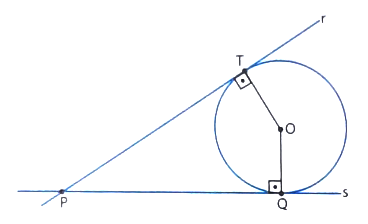
\includegraphics[width=1\linewidth]{imagens_8FMA108/imagem1}
    	
    	\noindent\textsubscript{~---------------------------------------------------------------------------}
    	\begin{enumerate}
    		\item Mostre que $\overline{PQ}$ e $\overline{PT}$, da figura anterior, são congruentes. \\\\\\\\\\\\\\\\\\\\\\\\\\\\\\\\\\\\
    		\item Na figura a seguir, $\overline{PT}$ é tangente à circunferência de centro $O$, e $\overline{AT}$ é um diâmetro dessa circunferência. Se a circunferência possui raio de medida 1,5 e $PA = 5$, calcule $PT$. 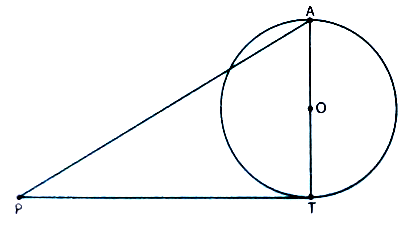
\includegraphics[width=1\linewidth]{imagens_8FMA108/imagem2}
    		 \newpage
    		\item Considere um ponto $P$ fora da circunferência de centro $O$ e diâmetro medindo 10 cm. Sendo $R$ e $T$ os pontos de tangência das semirretas $\stackrel{\longrightarrow}{PR}$ e $\stackrel{\longrightarrow}{PT}$ com a circunferência, como mostra a figura a seguir, e $PO = 13$ cm, calcule $PT$ e $PR$. 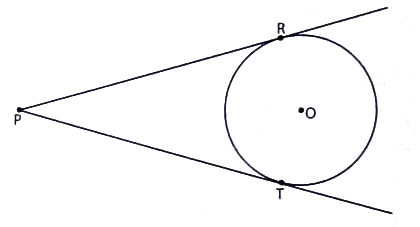
\includegraphics[width=1\linewidth]{imagens_8FMA108/imagem3} \columnbreak
    		
    		\item Mostre que qualquer triângulo inscrito numa circunferência será retângulo se um de seus lados for diâmetro da circunferência. \\\\\\\\\\\\\\\\\\\\
    		\item Usando régua e compasso, trace as tangentes ao círculo, passando pelo ponto externo $P$.
    		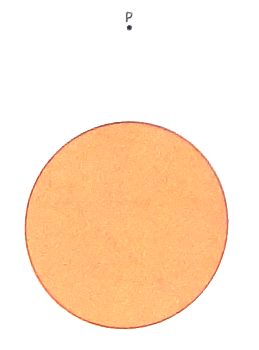
\includegraphics[width=1\linewidth]{imagens_8FMA108/imagem4}
    	\end{enumerate}
    $~$ \\ $~$ \\ $~$ \\ $~$ \\ $~$ \\ $~$ \\ $~$ 
    \end{multicols}
\end{document}